\documentclass{sprawozdanie-agh}

\usepackage[utf8]{inputenc}
\usepackage{listings}
\usepackage{tikz}
\usepackage{xcolor}
\usepackage{graphicx}
\usepackage{caption}
\usepackage{graphicx}
\usepackage{lipsum}
\usepackage{wrapfig}
\usepackage{subcaption}
\usepackage{accsupp}
\usepackage{array}
\usepackage{amsfonts}
\graphicspath{ {./img/} }

\usetikzlibrary{angles,quotes}
\makeatletter

\begin{document}

\przedmiot{Algorytmy geometryczne}
\tytul{Laboratorium 1}
\podtytul{Ćwiczenie wprowadzające}
\kierunek{Informatyka}
\autor{Kyrylo Iakymenko\\ Czwartek 13:00 - 14:30 tydzień B}
\data{Kraków, 16 października 2023}

\stronatytulowa{}

\section{Wprowadzenie}
\subsection{Cel ćwiczenia}
\quad To ćwiczenie ma na celu zapoznanie się z metodami generacji 
losowych punktów oraz badanie metod klasyfikacji położenia punktów na płaszczyźnie 
względem prostej. 
\subsection{Położenie punktu względem prostej}

\quad Położenie punktu względem prostej będziemy wyznaczać obliczjąc
dane wyznaczniki. Wyznaczniki pozwalają określić położenie
punktu c względem prostej która jest wyznaczona przez punkty a i b.
Jeżeli wyznacznik jest większy od 0 to punkt znajduje się z lewej strony prostej, jeżeli jest mniejszy
od 0  to
punkt znajduje się po prawej stronie prostej, a jeżeli wartość wyznacznika
jest równa 0 (lub jej wartość bezwzględna $< \varepsilon$) to punkt leży na prostej.

\quad Pomimo, że
powyższe wyznaczniki są sobie równoważne to na skutek
niedoskonałości reprezentacji liczb rzeczywistych w komputerze wyniki
mogą się różnić w zależności od użytego wyznacznika.

$$
(1)\det(a, b, c)= \begin{vmatrix}
       a_{x} - c_{x} & a_{y} - c_{y} \\
       b_{x} - c_{x} & b_{y} - c_{y} 
              \end{vmatrix}.\\
              $$
              $$
(2)\det(a, b, c) = \begin{vmatrix}
    a_x & a_y & 1\\
    b_x & b_y & 1\\
    c_x & c_y & 1
\end{vmatrix}.\\
$$
\section{Zbiory testowe}
\quad Na potrzeby ćwiczenia wygenerujemy $4$ zbiory punktów losowych.
\begin{enumerate}
    \item $10^5$ losowych punktów $(x, y)$ w przestrzeni $\mathbb{R}^2$, gdzie $(x, y) \in \left[-1000,1000\right]^{2}$.
    \item $10^5$ losowych punktów $(x, y)$ w przestrzeni $\mathbb{R}^2$, gdzie $(x, y) \in \left[-10^{14},10^{14}\right]^{2}$.
    \item $1000$ losowych punktów w przestrzeni $\mathbb{R}^2$ leżących na okręgu o środku $ O = (0,0)$ i promieniu $ R = 100$.
    \item $ 1000$ losowych punktów w przestrzeni $\mathbb{R}^2$ dla $ x \in \langle -1000,1000 \rangle$ leżących na prostej wyznaczonej przez wektor $ \overrightarrow{ab}$.   
    Gdzie $ a = (-1.0, 0.0)$, $ b = (1.0, 0.1)$.
\end{enumerate}

\section{Wykresy}
\begin{figure}[!h]
    \centering
    \begin{subfigure}{.5\textwidth}
      \centering
      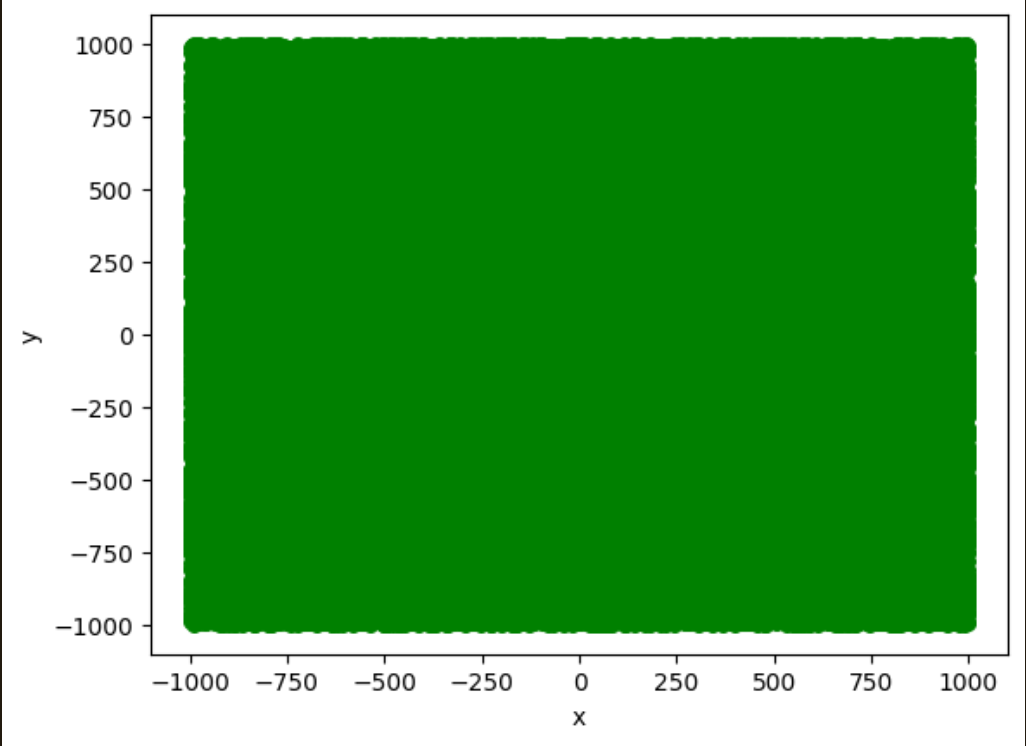
\includegraphics[width=.9\linewidth]{1.png}
      \caption*{Rys. 1: (a) $10^5$ losowych punktów $(x, y) \in \left[-1000,1000\right]^{2}$.}
      \label{fig:sub1}
    \end{subfigure}%
    \begin{subfigure}{.5\textwidth}
      \centering
      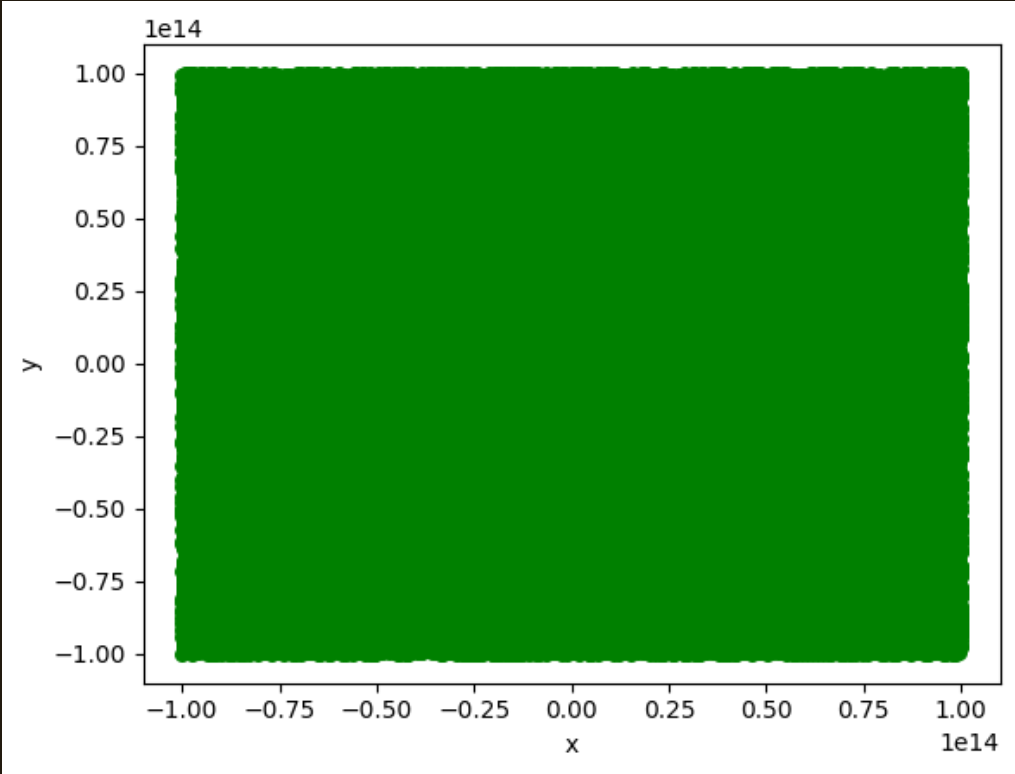
\includegraphics[width=.9\linewidth]{2.png}
      \caption*{Rys. 2: (b) $10^5$ losowych punktów $(x, y) \in \left[-10^{14},10^{14}\right]^{2}$.}
      \label{fig:sub2}
    \end{subfigure}
    \label{fig:test}
    \end{figure}
    \begin{figure}[!h]
    \centering
    \begin{minipage}{.5\textwidth}
      \centering
      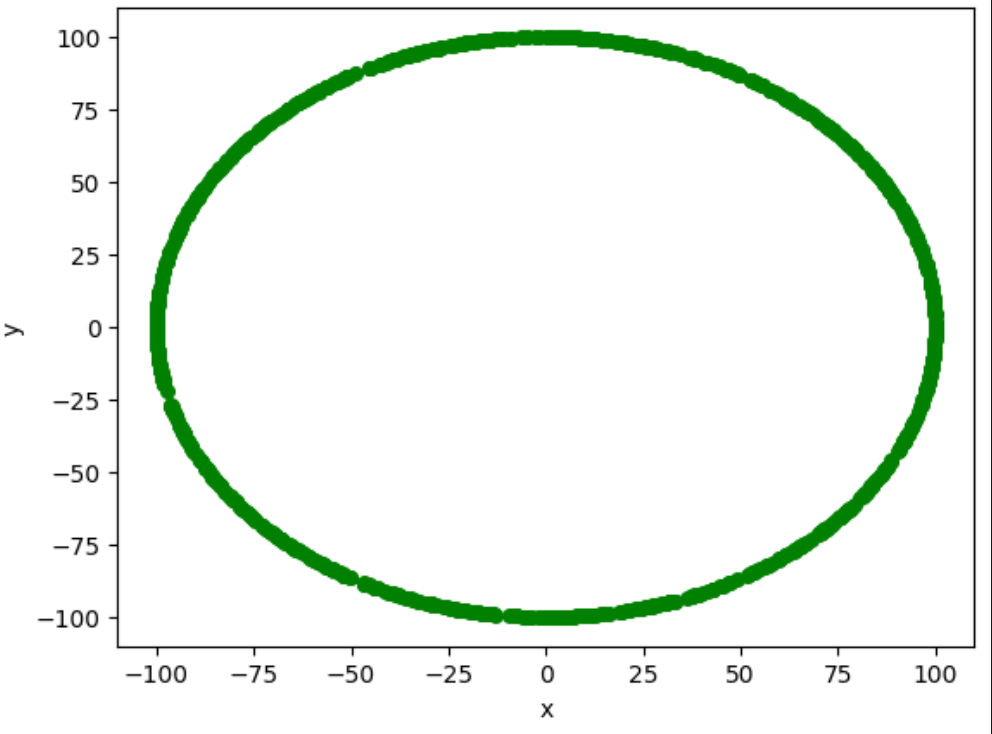
\includegraphics[width=.9\linewidth]{3.png}
      \caption*{Rys. 3: (c) $1000$ losowych punktów leżących na okręgu.}
      \label{fig:test1}
    \end{minipage}%
    \begin{minipage}{.5\textwidth}
      \centering
      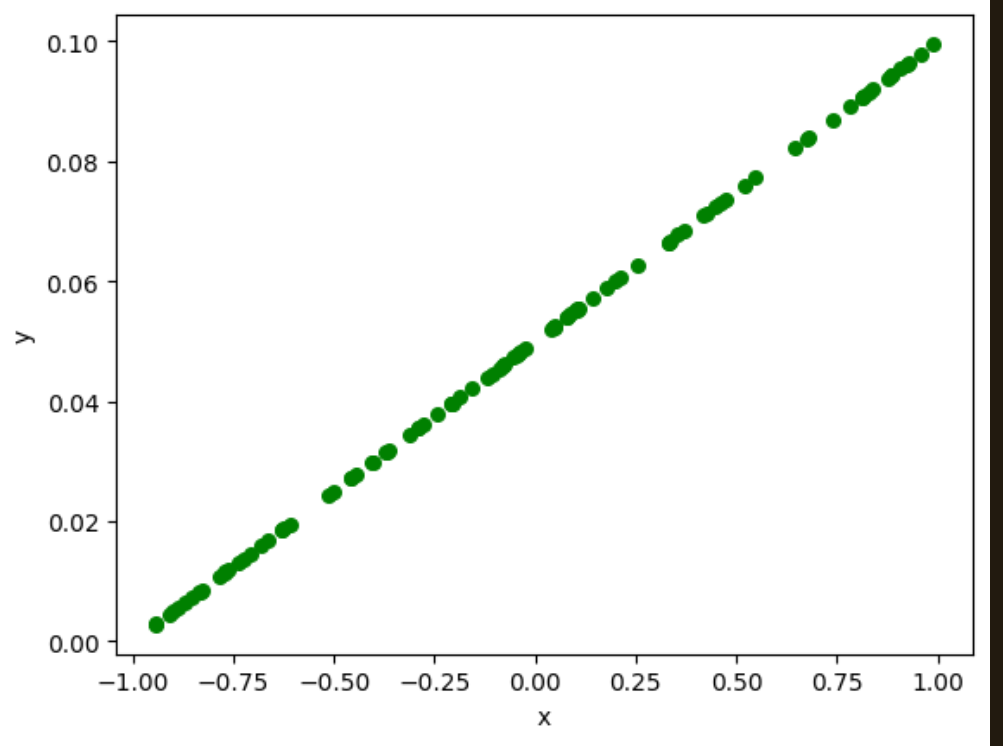
\includegraphics[width=.9\linewidth]{4.png}
      \caption*{Rys. 4: (d) $1000$ losowych punktów na prostej.}
      \label{fig:test2}
    \end{minipage}
    \end{figure}
\null
    \subsection{Algorytmy generacji zbiorów}
    \begin{enumerate}
    \item Dla zbiorów a i b. Osobna generacja każdego z $10^5$ losowych punktów.
    \item Dla zbioru c. Parametryzacja punktów na okręgu za pomocją funkcji trygonometrycznych $\sin$ i $\cos$.
    \item Dla zbioru d. Przekształcenie odcinka do postaci parametrycznej 
    $$
    l:\begin{cases}
      x = x_0 + tv_x& \smash{\raisebox{-1.6ex}{dla $\boldsymbol t \in [0,1]$.}}\\
      y = y_0 + tv_y
    \end{cases}
    $$
    A potem generowanie $t$ w podanym przedziale i dodanie odpowiednich punktów.
    \end{enumerate}
% \newpage



\section{Testy klasyfikacyjne dla różnych wartości $\varepsilon$}


\section{Porównywanie czasów klasyfikacji dla różnych funkcji obliczających wyznacznik}
\section{Testy precyzji float64 i float32}
\section{Podsumowanie}
\end{document}
